documentclass{standalone}
\usepackage{pgfplots}
\pgfplotsset{compat=newest}

\begin{document}
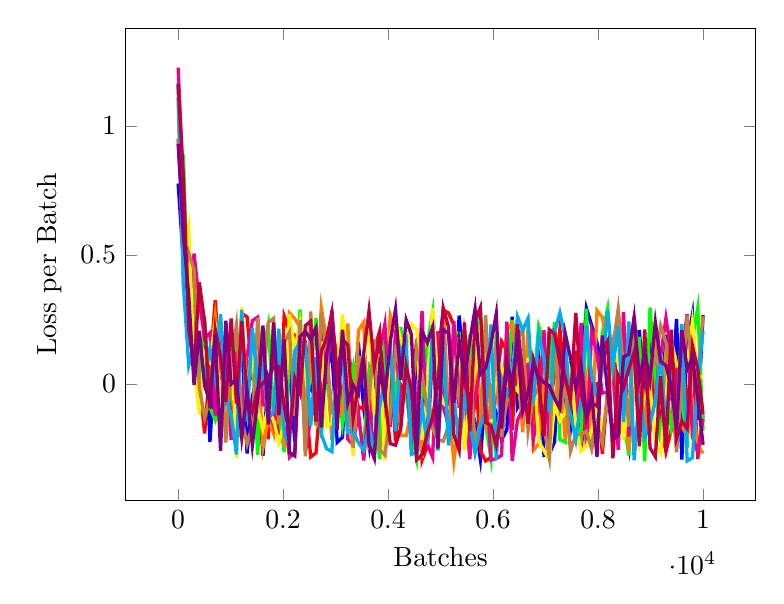
\begin{tikzpicture}
    \begin{axis}[width=8cm,height=6cm,xlabel={Batches},ylabel={Loss per Batch},scale only axis]
        \addplot [color=blue,very thick,mark=none,domain=1:10000,samples=100]{exp(-x/200)+rand*0.3};
        \addplot [color=red,very thick,mark=none,domain=1:10000,samples=100]{exp(-x/200)+rand*0.3};
        \addplot [color=green,very thick,mark=none,domain=1:10000,samples=100]{exp(-x/200)+rand*0.3};
        \addplot [color=orange,very thick,mark=none,domain=1:10000,samples=100]{exp(-x/200)+rand*0.3};
        \addplot [color=magenta,very thick,mark=none,domain=1:10000,samples=100]{exp(-x/200)+rand*0.3};
        \addplot [color=yellow,very thick,mark=none,domain=1:10000,samples=100]{exp(-x/200)+rand*0.3};
        \addplot [color=brown,very thick,mark=none,domain=1:10000,samples=100]{exp(-x/200)+rand*0.3};
        \addplot [color=cyan,very thick,mark=none,domain=1:10000,samples=100]{exp(-x/200)+rand*0.3};
        \addplot [color=purple,very thick,mark=none,domain=1:10000,samples=100]{exp(-x/200)+rand*0.3};
        \addplot [color=violet,very thick,mark=none,domain=1:10000,samples=100]{exp(-x/200)+rand*0.3};
    \end{axis}
\end{tikzpicture}
\end{document}